\documentclass{scrartcl}
\usepackage{mm_ws15}

\newcommand{\sheetTitle}{Blatt 7, Abgabe 8.12.2015, 12:00}
\begin{document}
\maketitle
\vspace{\baselineskip}

\textit{%
  Wir bereits angekündigt, wird am Freitag, den 11.12.2015 statt der Fragestunde eine Probeklausur abgehalten.
  Der Inhalt der Klausur wird sich nur über Themen erstrecken, die auf den Übungsblättern 1 -- 7 behandelt wurden.\\
  Die Teilnahme ist freiwillig und soll Ihnen ein Gefühl dafür geben, wie die Klausur am Ende des Semesters abläuft.
  Ihre Lösungen werden von uns korrigiert und in den Übungen am 17.12.2015 besprochen -- es wird deshalb kein Übungsblatt 8 in dieser Woche geben.
  Außerdem wird Ihnen ein Teil der erreichten Punkte in der Probeklausur als Zusatzpunkte für die Zulassung zur Klausur angerechnet.\\
}

\textbf{%
  Ohne gewichtigen Grund auf die Teilnahme zu verzichten ist Akt selbstmörderischen Wahnsinns.
  Nehmen Sie teil!\\
}

\textit{%
  In einer Vollversammlung am Donnerstag, den 3.12.15 um 14 Uhr in HS II informieren die Fachschaft über die Fachschaftsarbeit, was oder wen ihr wählen könnt, welche Gremien es gibt und wie ihr euch einbringen könnt.
  Außerdem werden die studentischen Mitglieder der Kommissionen in der Physik gewählt.\\
  Die Teilnehmer der Uebungsgruppe 2 (C. Christou) bitten wir sich auf andere Gruppen zum selben Termin zu verteilen
}

%%%%%%%%%%%%%%%%%%%%%%%%%%%%%%%%%%%%%%%%%%%%%%%%%%%%%%%%%%%%%%%%%%%%%%%%%%%%%%%%
\section{Flächenberechnung \& Volumenberechnung \points{5}}
\label{sec:flaechenberechnung}

\begin{subex}
  \item\points{2} Berechnen Sie das Integral
  \[
    I = \int_0^{1} \dd x \int_0^{1-x} \dd y .
  \]
  Überlegen Sie sich, was diese Integration geometrisch bedeutet.
  Was für eine Fläche beschreibt $I$?

  \item\points{3} Berechnen Sie das Volumen des Körpers $K = \{(x,y,z) \in \mathbb{R}^3 \, \vert \, x \in [-1, 1], x^2 + y^2 \le 1, 0 \le z \le 1 - \vert x \vert\}$ gegeben durch
  \[
    V
    = \int_{-1}^1 \dd x \int_{-\sqrt{1 - x^2}}^{\sqrt{1 - x^2}} \dd y \int_0^{1 - \vert x \vert} \dd z
    = 2 \int_{-1}^1 \dd x \, \sqrt{1 - x^2} \, (1 - \vert x \vert)
  \]
  indem Sie das eindimensionale Integral auf rechten Seite berechnen.
  Nutzen Sie die Symmetrie des Problems aus.
  Außerdem können Sie bereits bekannte Integrale benutzen.
  Begründen Sie außerdem die Wahl der Integrationsgrenzen des 3D Integrals.
\end{subex}


%%%%%%%%%%%%%%%%%%%%%%%%%%%%%%%%%%%%%%%%%%%%%%%%%%%%%%%%%%%%%%%%%%%%%%%%%%%%%%%%
\section{Substitution in Mehrfachintegralen \points{10}}
\label{sec:substitution_in_mehrfachintegralen}

Manche Mehrfachintegrale vereinfachen sich deutlich, wenn man eine Parametertransformation mehrerer Variablen gleichzeitig vornimmt.
In der Vorlesung haben Sie bereits Polarkoordinaten kennengelernt\footnote{%
  Die Definition der Vorlesung über den $\arctan$ gilt nur für $x > 0$.
  Diese kann man mit einer ähnlichen Fallunterscheidung (mit insgesamt 5 verschiedenen Fällen) auf alle $(x,y)$ erweitern.
}
\begin{equation}
  \label{eq:polar}
  r(x, y) = \sqrt{x^2 + y^2}, \quad\quad \phi(x, y) =
  \begin{cases}
    \arccos \frac{x}{\sqrt{x^2 + y^2}} & y \ge 0 \\ 2\pi - \arccos{\frac{x}{\sqrt{x^2 + y^2}}} & y < 0
  \end{cases}
\end{equation}

\begin{subex}
  \item\points{3} Was bedeuten diese beiden Gleichung geometrisch?
  Argumentieren Sie, dass die von den Koordinatenlinien $r$, $r+\Delta r$,  $\phi$, $\phi+\Delta \phi$ eingeschlossene Fläche für kleine $\Delta r$ und $\Delta \phi$ näherungsweise den Flächeninhalt $r \Delta r \Delta \phi$ hat.
  \item\points{3} Nutzen Sie das Ergebnis aus a) um das Volumen des Körpers $K$ aus Aufgabe~\ref{sec:flaechenberechnung} zu berechnen.
  Achten Sie insbesondere auf die neuen Integrationsgrenzen.
  \item\points{4} Benutzen Sie Polarkoordinaten um den Flächeninhalt der Menge
  \[
    C = \left\{ (x,y) \in \RR^2 \,\middle\vert\, (x^2 + y^2 + ax)^2 \le a^2 (x^2 + y^2) \right\}
  \]
  zu berechnen.
  Der Rand von $C$ ist in untenstehender Skizze dargestellt.
\end{subex}

\begin{center}
  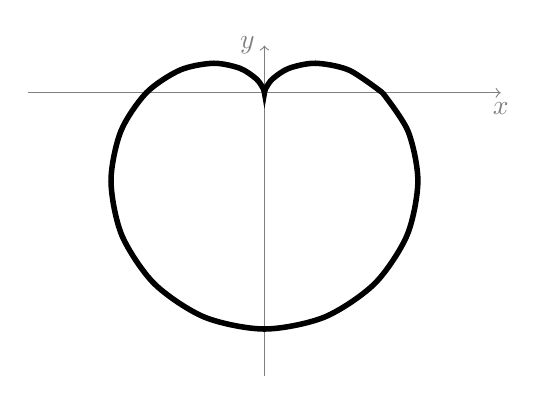
\begin{tikzpicture}[scale=1.5]
    \draw[gray,->] (-2,0) -- (2,0) node[below] {$x$};
    \draw[gray,->] (0,-2.4) -- (0,0.4) node[left] {$y$};
    \draw[domain=0:360,smooth,variable=\x,line width=2] plot ({(1 - sin(\x)) * cos(\x)},{(1 - sin(\x)) * sin (\x)});
  \end{tikzpicture}
\end{center}

\begin{remark}{Hinweis}
  Überlegen Sie sich die Umkehrung der Parametertransformation~\eqref{eq:polar}, d.h.\ bestimmen Sie $x(r,\phi)$ und $y(r,\phi)$.
  Wenn man diese in die Definitionsgleichung von $C$ einsetzt, bekommt man eine Bedingung für die Integrationsgrenzen heraus, die besonders einfach ist, wenn man zuerst über $r$ integriert.
\end{remark}


%%%%%%%%%%%%%%%%%%%%%%%%%%%%%%%%%%%%%%%%%%%%%%%%%%%%%%%%%%%%%%%%%%%%%%%%%%%%%%%%
\section{Komplexe Zahlen \points{8}}
\label{sec:komplexe_zahlen}

\begin{subex}
  \item\points{2} Bestimmen Sie Real- und Imaginärteil der folgenden komplexen Zahlen
  \[
    v = \frac{2 - 4\ii}{1 + 2\ii}, \quad\quad w = 3(3 - 2\ii), \quad\quad z = 2 \ee^{-\ii \frac{\pi}{4}}.
  \]
  \item\points{3} Berechnen Sie $v + w$, $v - w$, $vw$, $\frac{z}{w}$ und $\bar z$.
  Geben Sie die Lösung in der Form $u = \Re u + \ii\Im u$ an.
  \item\points{3} Finden Sie die Polarformel $z = r \ee^{\ii\Phi}$ für $v = 2 - 2\ii$ und $w_n = \ii^n$ ($n \in \mathbb{Z}$).
\end{subex}


%%%%%%%%%%%%%%%%%%%%%%%%%%%%%%%%%%%%%%%%%%%%%%%%%%%%%%%%%%%%%%%%%%%%%%%%%%%%%%%%
\section{Additionstheoreme \points{7}}
\label{sec:additionstheoreme}

Benutzen Sie \emph{Eulers Formel}
\[
  \ee^{\ii \phi} = \cos \phi + \ii \sin \phi
\]
um die folgenden Additionstheoreme zu beweisen.

\begin{subex}
  \item\points{2} $\sin(x + y) = \sin x \cos y + \cos x \sin y$
  \item\points{2} $\cos(x - y) = \cos x \cos y + \sin x \sin y$
  \item\points{3} $\sin x + \sin y = 2 \sin \frac{x + y}{2} \, \cos \frac{x - y}{2}$
\end{subex}


\end{document}
